\documentclass[a4paper,12pt]{article}
%For links
%\usepackage{url}
%For images
\usepackage{graphicx}
%For the "If, else" statment
\usepackage{amsmath}
\begin{document}
\begin{enumerate}
    \item



    \item
          Följande bild och beskrivning finns i en Volvo V70 instruktionsbok:
          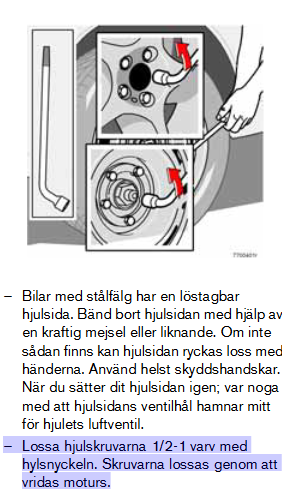
\includegraphics{Figur.png}

          Denna instruktion handlar om hur man lossar på ett hjul, men samma principer
          kan gå åt motsatt håll när man försöker dra åt
          Hylsnyckelns längd kan uppskattas till några decimeter, vi säger 2. Då gäller det att vrida
          bulten 1 varv, vilket krävs för att dra åt den helt.

          Då blir hävarmen runt 2 gånger kraften som man drar med. Ju hårdadre man drar destå
          mer hävarm.

    \item
          Vid kastbanans högsta punkt så är hastigheten för y axeln 0. Detta är för att
          kulan är precis vid sin maxpunkt och är påväg att börja åka neråt på grund utav
          graviationskraften.

          Istället kan endast hastigheten på x-axeln räknas ut enkelt så här:
          $22*cos(27^\circ)=20 m/s$ vilket då också är den totala hastigheten vid den punkten.

    \item
          För att simplifiera problemet kan man vinkla flaggstången så den liknar
          en gungbräda. Då får vi följande diagram:

          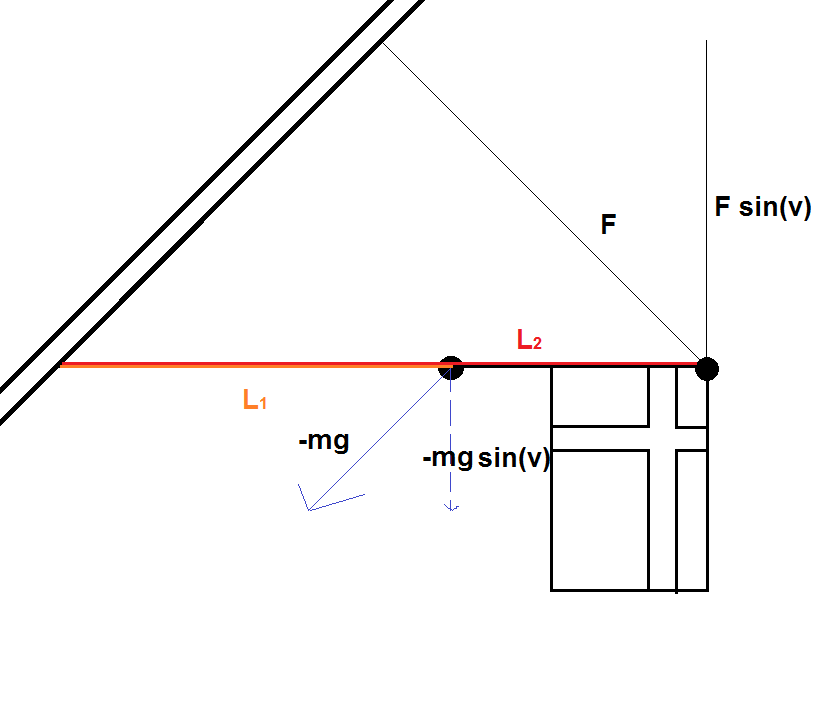
\includegraphics[scale=0.55]{Figur2.png}

          Flaggstången är i jämnvikt, så genom momentlagen får vi att summan av vridmomenten
          blir noll.

          $$FL_2sin(v)-mgL_1sin(v)=0$$
          $$FL_2=mgL_1$$
          $$F==\frac{mgL_1}{L_2}$$

          I uppgiften får vi reda på att massan på flaggstången är 53kg, Längden till
          tyngpunkten är 5 meter från punkten och att hela flaggstångens längd
          är 8.4 meter. Då får vi att F = 310 N.

    \item

          Man kan se att från perspektivet av Peter så accelererar myntet
          med motsatt acceleration som bussen.

          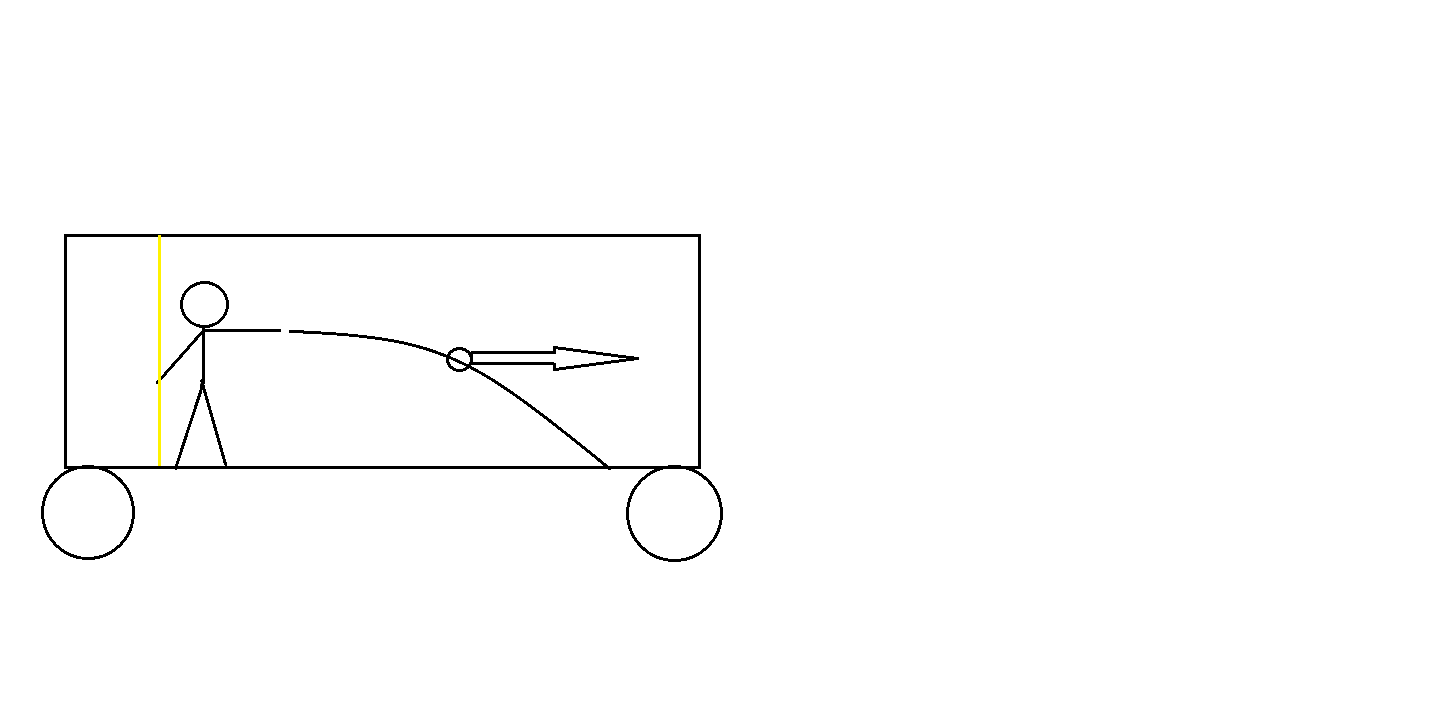
\includegraphics[scale=0.5]{Figur3.png}

          Då får vi att bollens x-position är

          $$x=x_0+v_0t+\frac{1}{2}at^2$$

          Men vi antar att $x_0=0$ och $v_0=0$.
          Ekvationen simplifieras då till

          $$x=\frac{1}{2}at^2$$

          Variabln som bör räknas ut är då t. Detta
          kan räknas ut i y-dimensionen där gravitationskraften
          drar ner myntet till golvet under en viss tid.

          $$y=y_0-\frac{1}{2}gt^2$$

          Den tiden det tar att landa på marken är när y=0,
          och ekvationen kan då skrivas om som

          $$t=\sqrt{\frac{2y_0}{g}}$$

          Då kombineras ekvationerna för x och y
          $$x=a\frac{y_0}{g}$$

          Med a=2.3, g=9.81 och y0=1.5 får man att
          myntet faller 0.35 meter bort. Men det finns anledningar
          till att tro att den skulle åka längre i verkligheten, för
          objekt kan studsa, rulla och glida, vilket dom här
          ekvationerna inte täcker.

\end{enumerate}
\end{document}